\documentclass{article}
\usepackage[utf8]{inputenc}
\usepackage{geometry}
\usepackage{graphicx}
\usepackage{hyperref}
\usepackage{titlesec}

\geometry{a4paper, margin=1in}

\titleformat{\section}{\large\bfseries}{\thesection}{1em}{}

\begin{document}

\title{Your Books List}
\author{Mohammed Serdar. 444004972.}
\date{October 2024}
\maketitle

\section*{Introduction}
It's an application to organize your books into lists based on your preferences.

\section*{Features}
\begin{itemize}
    \item \textbf{Access to all published books.}
    \item \textbf{Various sections} such as:
    \begin{itemize}
        \item Novel
        \item Scientific
        \item Psychological
        \item etc.
    \end{itemize}
    \item \textbf{Your lists are saved under your account.}
    \item \textbf{View your lists and book titles offline.}
    \item \textbf{Communicate with friends} by:
    \begin{itemize}
        \item Viewing each other's lists
        \item Suggesting books to each other
    \end{itemize}
    \item \textbf{Create public or private lists.}
\end{itemize}

\section*{Installation}
\begin{itemize}
    \item \textbf{Platforms:}
    \begin{itemize}
        \item Web
        \item Android
        \begin{itemize}
            \item Google Play
            \item Huawei AppGallery
        \end{itemize}
        \item Apple iOS
        \begin{itemize}
            \item App Store
        \end{itemize}
    \end{itemize}
\end{itemize}

\section*{User Guide}
\begin{itemize}
    \item \textbf{Sign-Up/Sign-In}
    \begin{itemize}
        \item By Email:
        \begin{enumerate}
            \item Create a username
            \item Enter your email
            \item Create a password
            \item On the sign-in page, enter your email and password
        \end{enumerate}
        \item By Google Account:
        \begin{enumerate}
            \item Click the Google button
            \item Choose the Google account to use in the app
        \end{enumerate}
    \end{itemize}
    \item \textbf{Home Page}
    \begin{itemize}
        \item Browse books
        \item View book sections
    \end{itemize}
    \item \textbf{Search Button}
    \begin{itemize}
        \item Search by:
        \begin{enumerate}
            \item Book title
            \item Author name
            \item ISBN
        \end{enumerate}
    \end{itemize}
    \item \textbf{Lists}
    \begin{itemize}
        \item Create a list
        \item Delete a list
    \end{itemize}
    \item \textbf{Settings}
\end{itemize}

\section*{Troubleshooting}
\begin{itemize}
    \item Adding a book to a list in offline mode:
    \begin{itemize}
        \item You need to be online, or the book won't be added.
    \end{itemize}
    \item If the list is private, others cannot view it.
    \item If you delete your account, all data will be gone.
\end{itemize}

\section*{Footnotes}
\begin{itemize}
    \item \href{https://a.storyblok.com/f/178313/491x424/0752fdbf6d/frame-415.webp}{App Page}
    \item \textbf{Another View:}
\end{itemize}

\begin{figure}[h]
    \centering
    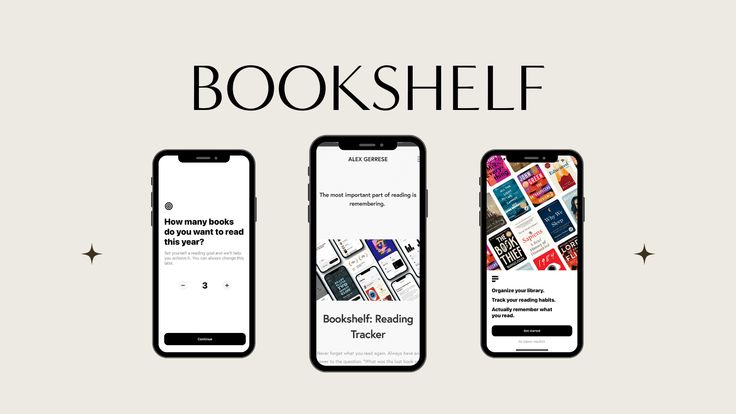
\includegraphics[width=0.5\textwidth]{image.jpg} 
    \caption{A view from the application}
\end{figure}

\end{document}
